% Options for packages loaded elsewhere
\PassOptionsToPackage{unicode}{hyperref}
\PassOptionsToPackage{hyphens}{url}
%
\documentclass[
]{article}
\usepackage{amsmath,amssymb}
\usepackage{lmodern}
\usepackage{iftex}
\ifPDFTeX
  \usepackage[T1]{fontenc}
  \usepackage[utf8]{inputenc}
  \usepackage{textcomp} % provide euro and other symbols
\else % if luatex or xetex
  \usepackage{unicode-math}
  \defaultfontfeatures{Scale=MatchLowercase}
  \defaultfontfeatures[\rmfamily]{Ligatures=TeX,Scale=1}
\fi
% Use upquote if available, for straight quotes in verbatim environments
\IfFileExists{upquote.sty}{\usepackage{upquote}}{}
\IfFileExists{microtype.sty}{% use microtype if available
  \usepackage[]{microtype}
  \UseMicrotypeSet[protrusion]{basicmath} % disable protrusion for tt fonts
}{}
\makeatletter
\@ifundefined{KOMAClassName}{% if non-KOMA class
  \IfFileExists{parskip.sty}{%
    \usepackage{parskip}
  }{% else
    \setlength{\parindent}{0pt}
    \setlength{\parskip}{6pt plus 2pt minus 1pt}}
}{% if KOMA class
  \KOMAoptions{parskip=half}}
\makeatother
\usepackage{xcolor}
\IfFileExists{xurl.sty}{\usepackage{xurl}}{} % add URL line breaks if available
\IfFileExists{bookmark.sty}{\usepackage{bookmark}}{\usepackage{hyperref}}
\hypersetup{
  pdftitle={Tillage and Cover Crop Mix Effects on Urban Soil Restoration},
  pdfkeywords={urban, compaction, cover crops},
  hidelinks,
  pdfcreator={LaTeX via pandoc}}
\urlstyle{same} % disable monospaced font for URLs
\usepackage[margin=1in]{geometry}
\usepackage{longtable,booktabs,array}
\usepackage{calc} % for calculating minipage widths
% Correct order of tables after \paragraph or \subparagraph
\usepackage{etoolbox}
\makeatletter
\patchcmd\longtable{\par}{\if@noskipsec\mbox{}\fi\par}{}{}
\makeatother
% Allow footnotes in longtable head/foot
\IfFileExists{footnotehyper.sty}{\usepackage{footnotehyper}}{\usepackage{footnote}}
\makesavenoteenv{longtable}
\usepackage{graphicx}
\makeatletter
\def\maxwidth{\ifdim\Gin@nat@width>\linewidth\linewidth\else\Gin@nat@width\fi}
\def\maxheight{\ifdim\Gin@nat@height>\textheight\textheight\else\Gin@nat@height\fi}
\makeatother
% Scale images if necessary, so that they will not overflow the page
% margins by default, and it is still possible to overwrite the defaults
% using explicit options in \includegraphics[width, height, ...]{}
\setkeys{Gin}{width=\maxwidth,height=\maxheight,keepaspectratio}
% Set default figure placement to htbp
\makeatletter
\def\fps@figure{htbp}
\makeatother
\setlength{\emergencystretch}{3em} % prevent overfull lines
\providecommand{\tightlist}{%
  \setlength{\itemsep}{0pt}\setlength{\parskip}{0pt}}
\setcounter{secnumdepth}{-\maxdimen} % remove section numbering
\newlength{\cslhangindent}
\setlength{\cslhangindent}{1.5em}
\newlength{\csllabelwidth}
\setlength{\csllabelwidth}{3em}
\newlength{\cslentryspacingunit} % times entry-spacing
\setlength{\cslentryspacingunit}{\parskip}
\newenvironment{CSLReferences}[2] % #1 hanging-ident, #2 entry spacing
 {% don't indent paragraphs
  \setlength{\parindent}{0pt}
  % turn on hanging indent if param 1 is 1
  \ifodd #1
  \let\oldpar\par
  \def\par{\hangindent=\cslhangindent\oldpar}
  \fi
  % set entry spacing
  \setlength{\parskip}{#2\cslentryspacingunit}
 }%
 {}
\usepackage{calc}
\newcommand{\CSLBlock}[1]{#1\hfill\break}
\newcommand{\CSLLeftMargin}[1]{\parbox[t]{\csllabelwidth}{#1}}
\newcommand{\CSLRightInline}[1]{\parbox[t]{\linewidth - \csllabelwidth}{#1}\break}
\newcommand{\CSLIndent}[1]{\hspace{\cslhangindent}#1}
\usepackage{booktabs}
\usepackage{longtable}
\usepackage{array}
\usepackage{multirow}
\usepackage{wrapfig}
\usepackage{float}
\usepackage{colortbl}
\usepackage{pdflscape}
\usepackage{tabu}
\usepackage{threeparttable}
\usepackage{threeparttablex}
\usepackage[normalem]{ulem}
\usepackage{makecell}
\usepackage{xcolor}
\ifLuaTeX
  \usepackage{selnolig}  % disable illegal ligatures
\fi

\title{Tillage and Cover Crop Mix Effects on Urban Soil Restoration}
\author{true \and true \and true}
\date{}

\begin{document}
\maketitle
\begin{abstract}
Urban soils are highly disturbed, resulting in the loss of vegetation, organic matter, and increased compaction. Urban farmers rely on compost to improve degraded soil, but an integrated strategy may enhance soil quality more than simply apply compost. This study examined how various tillage methods and cover crop mixes affected soil attributes such as compaction, water infiltration rate, herbaceous weedy plant emergence, and crop yield. Tractor tilled plots relieved compaction to significantly greater depths compared to no-till (minimal disturbance) and roto-tilled (moderate disturbance) plots. Roto-tilled soils infiltrated water at a higher rate rate than the no-till and tractor tilled soils, challenging cited benefits expected from extensive tillage. Cover crops varied in yield across tillage treatments and the average root mass of forage radish was greater no-till plots but not significantly different, despite that tillage group having lower water infiltration rates and higher compaction. The weed suppression cover crop mix (sorghum-sudangrass, buckwheat, and cowpea) had fewer weeds than the other two cover crop mixes. We posit that integrated approaches to soil management tailoring tillage to crop use can improve soil function better than simply adding compost.
\end{abstract}

{
\setcounter{tocdepth}{2}
\tableofcontents
}
Journals: Elsevier--Soil \& Tillage Research (IF=5), Urban Forestry \& Urban Greening (1wk), or then Wiley--ASA Agronomy Journal (?), Ecology \& Evolution (replicates), or lastly PCI Ecology submission (45d) w/ pre-print archived in agriRxiv, ecoEvoRxiv, or bioRxiv.

\hypertarget{introduction}{%
\section{Introduction}\label{introduction}}

Urban soils have the potential to improve the livelihoods of most of the world \emph{(\protect\hyperlink{ref-ref}{\textbf{ref?}})} via implications for climate adaptation, erosion and storm-water runoff management, and local forestry \emph{(\protect\hyperlink{ref-payao-zuckerman08}{\textbf{payao-zuckerman08?}})}, but many urban soils are in poor health for cultivation after decades of industrial use, including sealing and structural engineering \emph{(\protect\hyperlink{ref-oldeman91}{\textbf{oldeman91?}})}.
This is especially notable in post-industrial cities of the mid-western USA, where many vacant lots remain on soils can have relatively high compaction, pH, and chemical contamination \emph{(\protect\hyperlink{ref-beniston11}{\textbf{beniston11?}})}.
Degraded urban soils with low organic matter are also likely far from organic carbon saturation \emph{(\protect\hyperlink{ref-stewart07}{Stewart et al. 2007})}, making the potential response to tailored agricultural management large \emph{(\protect\hyperlink{ref-kumar16}{Kumar and Hundal 2016}; \protect\hyperlink{ref-kuzyakov19}{Kuzyakov and Zamanian 2019})}.
However, popular single strategies like organic compost amendments to urban gardens, while widely beneficial across many physical, chemical, and biological properties \emph{(\protect\hyperlink{ref-refs}{\textbf{refs?}})}, can also have other side effects like excess phosphorus \emph{(\protect\hyperlink{ref-small19}{Small et al. 2019})}, which highlights the benefits of new and ongoing research studies of urban soil management, especially of integrated approaches for soil multifunctionality \emph{(\protect\hyperlink{ref-blesh17}{\textbf{blesh17?}})} including cover cropping, tillage, diverse mulching, and others.
In response to various needs, urban agriculture continues to expand as local communities and non-profit organizations revitalize and establish a diversity of new green initiatives including landscaping to improve local access to healthy food and a cleaner and safer environment \emph{(\protect\hyperlink{ref-heckler12}{\textbf{heckler12?}})}.
Urban growers in particular often invest relatively large amounts of money, time, and resources from accessible capital into amending soils for vegetable production \emph{(\protect\hyperlink{ref-ref}{\textbf{ref?}})},
thereby improving the potential impact of research for promising accessible urban soil remediation strategies, which remains limited beyond compost \emph{(\protect\hyperlink{ref-ref}{\textbf{ref?}})}.

\hfill\break

Mechanized tilling has long been a regular strategy improve short-term arability \emph{(\protect\hyperlink{ref-badalikova09}{\textbf{badalikova09?}})}, among others like adding compost, although research studies increasingly report soil degradation after long-term and intensive tillage \emph{(\protect\hyperlink{ref-refs}{\textbf{refs?}})}.
Short-term tillage benefits include larger soil pores and lower soil bulk density \emph{(\protect\hyperlink{ref-hill85}{\textbf{hill85?}})}, and more available nutrients \emph{(\protect\hyperlink{ref-ref}{\textbf{ref?}})} yet less weed regeneration \emph{(\protect\hyperlink{ref-ref}{\textbf{ref?}})}, making tillage useful against soil compaction and associated water infiltration and drainage issues, which facilitates faster seeding and crop establishment early in the season \emph{(\protect\hyperlink{ref-ref}{\textbf{ref?}})}.
However, longer-term side effects of excessive and/or very intensive tillage include weaker soil structure \emph{(\protect\hyperlink{ref-catania18}{\textbf{catania18?}})}, increasing dependence on tillage to maintain past yields \emph{(\protect\hyperlink{ref-ref}{\textbf{ref?}})}, \ldots{}\emph{(\protect\hyperlink{ref-ref}{\textbf{ref?}})} and faster soil erosion \emph{(\protect\hyperlink{ref-handelsman21}{\textbf{handelsman21?}})}, which has more recently led to events like the USA Dust Bowl \emph{(\protect\hyperlink{ref-ref}{\textbf{ref?}})}, and historically poses an existential threat to agricultural societies when combined with other stressors \emph{(\protect\hyperlink{ref-montgomery07}{Montgomery 2007})}.
In response, sustainable and regenerative agriculture movements advise no-till or minimal-till management approaches, like broadfork tools, to re-focus on soil health and fertility \emph{(\protect\hyperlink{ref-xiao-bin06}{\textbf{xiao-bin06?}}; \protect\hyperlink{ref-roger-estrade10}{\textbf{roger-estrade10?}})}, which comes with different challenges like stronger pressure from weeds \emph{(\protect\hyperlink{ref-ref}{\textbf{ref?}})}, highlighting a role for continuing research into diverse no-till strategies.
For urban growers, machinery can also be cost-prohibitive, and limited access to agricultural loans \emph{(\protect\hyperlink{ref-USDA}{\textbf{USDA?}})} has resulted in affected communities adapting by organizing equipment sharing systems, which can be more practical in denser urban housing arrangements compared to diffuse rural ones.
This variation in accessibility of machinery can promote mixed tillage strategies by urban growers including tractor- and/or roto-till, which likely have different effects on soil and weed issues, but there remains little public documentation comparing benefits of various tillage styles on remediating urban soils \emph{(\protect\hyperlink{ref-ref}{\textbf{ref?}})}, which slows the innovation of tailored management strategies for the array of urban grower goals.

\hfill\break

Cover cropping has been another long-recommended strategy of sustaining longer-term yields by maintaining soil fertility \emph{(\protect\hyperlink{ref-carverux2fwhite}{\textbf{carver/white?}}; \protect\hyperlink{ref-handelsman}{\textbf{handelsman?}})}, although current strategies could be improved from relying on single species to designing complementary species mixes.
The namesake benefit of cover crops is to cover the soil in areas without active cultivation, which maintains root activity and weakens erosion \emph{(\protect\hyperlink{ref-ref}{\textbf{ref?}})}, but different species will also vary in the benefits they can provide based on physiological traits.
For example, legumes like cowpea (or black-eyed peas, \emph{Vigna unguiculata}), clovers (\emph{Trifolium sp.}), and hairy vetch (\emph{Vicia villosa}) are popular cover crops because of their additional symbioses with root bacteria that fix nitrogen from the air into soils where it is more available for future crop use \emph{(\protect\hyperlink{ref-grossman}{\textbf{grossman?}})}.
Similarly, buckwheat helps scavenge soil phosphorus \emph{(\protect\hyperlink{ref-SAREguide}{\textbf{SAREguide?}})}, which is often a limiting macro-nutrient in the tropics \emph{(\protect\hyperlink{ref-ref}{\textbf{ref?}})}, and could also be combined with compost that is usually high in phosphorus to address a recurring soil phosphorus deficiency.
Other plants, including grasses like sorghum, tend to grow deep roots, or have other traits like chemical defenses named allelopathy, that compete with weeds enough to keep them suppressed over time \emph{(\protect\hyperlink{ref-SAREguide}{\textbf{SAREguide?}})}.
Broader implications of cover cropping also include higher soil organic matter, though the underlying processes remain complex \emph{(\protect\hyperlink{ref-king20}{King et al. 2020})}, and few studies show direct correlations \emph{(\protect\hyperlink{ref-oldfield19}{Oldfield, Bradford, and Wood 2019})}.
Furthermore, while large rural organic farms can benefit from incorporating specifically-chosen cover cropping into their mechanized operations, the reliance of urban agriculture more on labor over machinery offers an opportunity to develop new cover cropping systems that combine seeding and terminating different species together to improve the potential efficiency of soil remediation efforts.
For example, sorghum, cowpea, and buckwheat could be combined into a mixed strategy that can increase soil nitrogen, soil phosphorus, and suppress weeds via deep and shallow roots with allelopathic chemical defenses, although cover crop synergisms remain understudied \emph{(\protect\hyperlink{ref-ref}{\textbf{ref?}})}.
An integrated complex approach to optimizing cover cropping systems including interspecific species interactions are well-posed to be initially researched in urban agriculture and followed by later adaptation to rural agriculture as well \emph{(\protect\hyperlink{ref-nationalSciTechCouncil17}{\textbf{nationalSciTechCouncil17?}})}.

\hfill\break

In this study, we investigated how different tillage techniques and cover crop species mixes affect soil physical properties and yield {[}over the course of one growing season{]}.
The tillage methods ranged from high disturbance using a tractor and implements to minimal disturbance with a broadfork.
Cover crop species mixes were selected based on target functions including reducing compaction, suppressing weeds, and perenniality, or potential for sustainable re-growth.
We hypothesized that the benefits of tillage and cover crop mixing would be interchangeable, meaning that both tillage and cover crop mixes could improve soil compaction and suppress weeds to similar degrees, also increasing yield.
Accordingly, we predicted that roto-till, a moderate soil disturbance, would best balance compaction and weed pressure benefits, deepening where soil hardpan layers occur that limit root penetration, increasing soil water infiltration rates, and reducing weed cover, density, and diversity.
We also expected that the cover crop mix designed against soil compaction would have the deepest soil harpan depth and highest water infiltration rates compared to other mixes, due to the strong rooting by selected radish and ryegrass species.
Finally we expected that the cover crop mix designed for weed suppression would experience the lowest local weed cover, density, and diversity, due to allelopathic chemical defense traits.

\hypertarget{methods}{%
\section{Methods}\label{methods}}

\begin{verbatim}
## -- Attaching packages --------------------------------------- tidyverse 1.3.1 --
\end{verbatim}

\begin{verbatim}
## v ggplot2 3.3.6     v purrr   0.3.4
## v tibble  3.1.7     v dplyr   1.0.9
## v tidyr   1.2.0     v stringr 1.4.0
## v readr   2.1.2     v forcats 0.5.1
\end{verbatim}

\begin{verbatim}
## -- Conflicts ------------------------------------------ tidyverse_conflicts() --
## x dplyr::filter() masks stats::filter()
## x dplyr::lag()    masks stats::lag()
\end{verbatim}

\begin{verbatim}
## here() starts at /Users/nicholasmedina/Documents/u/0/art/res/GitHub/must
## here() starts at /Users/nicholasmedina/Documents/u/0/art/res/GitHub/must
\end{verbatim}

\begin{verbatim}
## 
## Attaching package: 'rstatix'
\end{verbatim}

\begin{verbatim}
## The following object is masked from 'package:stats':
## 
##     filter
\end{verbatim}

\begin{verbatim}
## Rows: 324 Columns: 12
## -- Column specification --------------------------------------------------------
## Delimiter: ","
## chr (4): SAMPL_TIME, COL, TIL, MIX
## dbl (8): ROW, PND, INFIL_OZ.SEC, TOTRAD_oz, RADL_CM, Wd_Abn, Wd_Dn, Wd_Cov
## 
## i Use `spec()` to retrieve the full column specification for this data.
## i Specify the column types or set `show_col_types = FALSE` to quiet this message.
## `summarise()` has grouped output by 'SAMPL_TIME', 'MIX', 'TIL', 'COL'. You can override using the `.groups` argument.
\end{verbatim}

\hypertarget{study-site}{%
\section{Study site}\label{study-site}}

The study site was located at the Michigan State University (MSU) - Detroit Partnership for Food, Learning, and Innovation (DPFLI) (42.4, -83.3), a 1.6-ha (4 acres) extension facility dedicated to urban agriculture and engaging with local small-scale growers in Detroit, MI, USA.
The climate is temperate with four seasons, with mean annual temperature of \textasciitilde9.5 C (49.1 F) and precipitation at \textasciitilde{} mm (31 in) \emph{(\protect\hyperlink{ref-ref}{\textbf{ref?}})}.
The site was formerly a school building and associated playground until 2016 when it was demolished \textbf{after closing for \ldots{} reasons} and the land became vacant.
The habitat is \textasciitilde1.2 km (\textasciitilde0.8 mi) away from a small river, conferring some wetland ecosystem properties like denser soils.
It is also surrounded by sealed sidewalk and small roads on all four sides, which likely affects runoff and drainage patterns (Fig \ref{fig:plots}).
\includegraphics{merge_files/figure-latex/plots-1.pdf}

The soils can be classified as Technosols, given that large metal artifacts can be found throughout various profiles \emph{(\protect\hyperlink{ref-fao14}{\textbf{fao14?}})}, from when the area was filled in with nearby soils during highway road construction, as was common in mid-western USA industrial manufacturing cities many decades ago in the \emph{1960s} \emph{(\protect\hyperlink{ref-beniston16}{Beniston, Lal, and Mercer 2016})}.
Accordingly, the growing area has both a finer- and coarser-textured side \emph{(\protect\hyperlink{ref-USDA-NRCSwebsoilsurvey}{\textbf{USDA-NRCSwebsoilsurvey?}}--designPlots??)},
and this study was done on the side with consistent clay \textasciitilde37\% (\ref{fig:plots}).
Topsoil A horizons are 1-2'' (\textless5 cm) deep, and subsoil B horizons can be \textgreater30.5 cm (1 ft) deep, with a muted yellow color \emph{YR\#\#?!} (\ref{fig:plots}).
A baseline site-level soil lab assessment from Cornell determined that the top 4'' (10 cm) of soils around the site together have relatively good organic matter at \textasciitilde{} ± \% and nutrient levels, including those of heavy metals like lead and arsenic \emph{(Table ???)} which were present below harmful government human-contact standards \emph{(\protect\hyperlink{ref-angelone02}{\textbf{angelone02?}}; \protect\hyperlink{ref-EPA}{\textbf{EPA?}})}, as well as decent but sub-optimal \textasciitilde, CO, 2 respiration rates of ± mg per day (Table \ref{tab:chem}.
Some main concerns limiting productivity include high alkaline pH of 463.6 ± 24.9 lowering availability of existing nutrients, as well as weak aggregate stability of ± leading to issues with aeration, infiltration, rooting, crusting when dry, erosion, and runoff (Table \ref{tab:chem}).

\hypertarget{study-design}{%
\subsection{Study design}\label{study-design}}

The study area was a 278 \emph{m\textsuperscript{2}} (2992.4 \emph{ft\textsuperscript{2}}) section on the East side of the site that was divided into 36 separate 4.6 \emph{m\textsuperscript{2}} (49.5 \emph{ft\textsuperscript{2}}) plots in nine rows and four columns (Fig \ref{fig:plots}).
Tillage groups spanned the nine columns in adjacent groups of three, while cover crop mix treatments spanned the rows with one row per cover crop mix, which totaled 12 plots per tillage group and nine plots per cover crop mix.
Before applying treatments, approximately 0.2 \emph{m\textsuperscript{3}} (8.5 \emph{ft\textsuperscript{3}}) of compost was incorporated into each plot.

\emph{One aggregated sample per tillage group was collected and analyzed for chemistry using modified Morgan-extractable protocols at the MSU soil test lab (\protect\hyperlink{ref-moebius-clune16}{\textbf{moebius-clune16?}}) and analysis was also conducted on the compost.}

\hypertarget{tillage}{%
\subsection{Tillage}\label{tillage}}

These methods represent a spectrum of soil management practices used and potentially available for small scale agriculture.
Specifically we tested three tillage techniques:
1) no-till with a broadfork (NT),
2) moderate intensity with a roto-tiller (RT), and
3) intensive tractor-till (TT) with implements.
Tractor-till plots were worked with a subsoiler, moldboard plow, and rototiller attached to a tractor up to 30.5 cm (1 ft) deep.
RT plots were tilled with a rototiller implement up to 20 cm (7.9 in) deep.
NT plots were worked with a broadfork up to 10 cm (3.9 in) deep.
These treatments were selected based on varying tillage philosophies, costs of implementation, and degree of mechanization.

\hypertarget{cover-crop-mixes}{%
\subsection{Cover crop mixes}\label{cover-crop-mixes}}

Cover crop mixes were designed based on plants associated with targeted benefits.
We tested the performance of three mixes, each composed of three different plant species (Table \ref{tab:crops}).
The compaction mix focused on plants with roots that tend to penetrate and loosen soil well, specifically crimson clover (\emph{Trifolium incarnatum}), forage radish (\emph{Raphanus sativus}), and cereal ryegrass (\emph{Secale cereale}) \emph{(\protect\hyperlink{ref-williamsux2fweil04}{\textbf{williams/weil04?}})}.
The weed suppression mix consisted of heat- and drought-tolerant crops that grow rapidly, allowing them to outcompete other plants \emph{(\protect\hyperlink{ref-ref}{\textbf{ref?}})}, specifically sorghum-sudangrass (\emph{Sorghum bicolor x Sorghum bicolor var. sudanese}), cowpea (\emph{Vigna unguiculata subsp. unguiculata}), and buckwheat (\emph{Fagopyrum esculentum}).
Lastly, the perennial mix was made up of plants that would survive beyond one growing season and return in the spring, adding additional biomass and outcompeting early season weeds \emph{(\protect\hyperlink{ref-ref}{\textbf{ref?}})}, specifically hairy vetch (\emph{Vicia villosa}), red clover (\emph{Trifolium pratense}), and wheat (\emph{Triticum aestivum}).
We also had a null control group consisting of established vegetation within the plot, where no additional seeds were sown.

\begin{verbatim}
## ==  1 queries  ===============
## ✔  Found:  Hairy+Vetch[Common Name]
## ==  Results  =================
## 
## • Total: 1 
## • Found: 1 
## • Not Found: 0
## ==  1 queries  ===============
## ✔  Found:  Red+Clover[Common Name]
## ==  Results  =================
## 
## • Total: 1 
## • Found: 1 
## • Not Found: 0
## ==  1 queries  ===============
## ✔  Found:  Wheat[Common Name]
## ==  Results  =================
## 
## • Total: 1 
## • Found: 1 
## • Not Found: 0
## ==  1 queries  ===============
## ==  Results  =================
## 
## • Total: 1 
## • Found: 0 
## • Not Found: 0
## ==  1 queries  ===============
## ✔  Found:  Black-Eyed+Pea[Common Name]
## ==  Results  =================
## 
## • Total: 1 
## • Found: 1 
## • Not Found: 0
\end{verbatim}

\begin{table}

\caption{\label{tab:crops}Cover crop mixes}
\centering
\begin{tabular}[t]{l|l|l}
\hline
Function & Plants & Binomial\\
\hline
Null & Existing vegetation (no manipulation) & \\
\cline{1-2}
 & Hairy Vetch & \\
\cline{2-2}
 & Red Clover & \\
\cline{2-2}
\multirow{-3}{*}{\raggedright\arraybackslash Perennial} & Wheat & \\
\cline{1-2}
 & Forage Radish & \\
\cline{2-2}
 & Crimson Clover & \\
\cline{2-2}
\multirow{-3}{*}{\raggedright\arraybackslash Compaction} & Cereal Ryegrass & \\
\cline{1-2}
 & Sorghum-Sudangrass & \\
\cline{2-2}
 & Cowpea & \\
\cline{2-2}
\multirow{-3}{*}{\raggedright\arraybackslash Weed Suppression} & Buckwheat & \multirow{-10}{*}{\raggedright\arraybackslash NA}\\
\hline
\end{tabular}
\end{table}

\hypertarget{data-collection}{%
\subsection{Data Collection}\label{data-collection}}

\hypertarget{compaction}{%
\subsubsection{Compaction}\label{compaction}}

Soil compaction was measured with a penetrometer \emph{(AgraTronix, Soil Compaction Tester \#08180)} in four randomly selected spots within each quarter of every plot, which were later averaged at the plot level.
Individual measurements were recorded as the depth at which the penetrometer read 2 MPa (290.1) pounds per square inch or psi), since roots typically cannot penetrate with 2 MPa of force \emph{(\protect\hyperlink{ref-duiker02}{\textbf{duiker02?}})}.
Sampling was conducted at two separate time periods, in July (``Early'') and October (``Late'') 2019.
Samples were taken on dry days and recorded to the nearest inch.

\hypertarget{infiltration}{%
\subsubsection{Infiltration}\label{infiltration}}

We measured the water infiltration rate to determine the soil's capacity to drain water, which has implications for managing storm-water runoff and holding water for plant roots.
The infiltration rate was calculated by recording the amount of time it took for \textasciitilde1 L (32 fl oz) to drain into the soil, which is similar to the amount of typical rainfall on \textasciitilde0.10 \emph{m\textsuperscript{2}} (\textasciitilde1 \emph{ft\textsuperscript{2}}) per rain event \emph{(\protect\hyperlink{ref-USGS}{\textbf{USGS?}})}.
For each plot we cleared the soil surface of debris and cut vegetation low enough to explose the surface.
Then we pressed an empty \textasciitilde1.4 kg (48 oz) aluminum can \textasciitilde2.5 cm (1 in) into the soil and poured the water in.
The maximum time allowed was 160 seconds \textbf{recorded as\ldots??}.

\hypertarget{weed-cover-density-and-richness}{%
\subsubsection{Weed cover, density, and richness}\label{weed-cover-density-and-richness}}

We recorded three measures of weed activity that described overall weed pressure in different ways.
Weed cover was estimated as the proportion of total area covered by all weed species combined within a plot, using a scale of 1-10 with one indicating \textbf{only one species / near zero stems} observed to 10 being \textbf{10 species present / almost the entire plot surface covered at some level with at least part of a weed plant (e.g.~stem or leaf)}.
Weed richness was measured by counting the total number of morphologically distinguishable weedy plants with at least one individual stem observed in a plot.
Weed density was measured as the \textbf{number of individual stems / relative cover} of either of the two most abundant weed species -- pigweed (\emph{Palmer amaranth / Amaranthus viridis}) and velvetleaf (\emph{Abutilon theophrasti}) -- using a discrete scale in increments of 10 with 0 indicating neither species present and 5 indicating 50 or more total individuals stems of either species.

\hypertarget{yield}{%
\subsubsection{Yield}\label{yield}}

Five forage radish (\emph{Raphanus sativus}) roots were randomly selected from each plot and measured for length, individually, and wet weight, as a cluster.
The length of a radish root was measured from the hypocotyl, or root cap, to where the root became \textasciitilde6.3 mm (\textasciitilde1⁄4 in) wide.

\hypertarget{statistical-analyses}{%
\subsection{Statistical analyses}\label{statistical-analyses}}

All data were centered using plot-level medians and run through Kruskal-Wallis tests, which are non-parametric and so make minimal assumptions about underlying distributions, making them relatively generalized and suitable for data with less replication.
Since these tests are limited in model formulation complexity, tests analyzing tillage and cover crop treatments were run separately, as reflected in the design of results figures.
In cases where a treatment category was significant overall, pairwise Wicoxon tests between all individual treatment pairs were run post-hoc to determine specific differences underlying the overall treatment effect, with Holm corrections to p-values for multiple comparisons.
Data were also pooled across sample times given no significant effect on data, to increase statistical power under these statistical model conditions, for all variables except infiltration rate.
Tillage by cover crop analyses were not done for infiltration and yield, since infiltration data was taken from only \textbf{\#\#\#\#} plots, and yield data came from only compaction plots.
All calculations and analyzes were done in R version 4.2.0 (2022-04-22) mainly using the packages \emph{tidyverse} 1.3.1 \emph{(\protect\hyperlink{ref-ref}{\textbf{ref?}})} and \emph{rstatix} 0.7.0 \textbf{(\protect\hyperlink{ref-ref}{\textbf{ref?}})}.
Data and code are stored at \url{nmedina17.github.com/must}.

\hypertarget{results}{%
\section{Results}\label{results}}

\hypertarget{compaction-1}{%
\subsection{Compaction}\label{compaction-1}}

Compaction was affected significantly overall by tillage treatments (\emph{p} = \textless0.0001) across cover crop treatments (Fig \ref{fig:compactFig}).
Tractor-till had the largest significant effect on depth to hardpan compared to no-till (\emph{p} = \textless0.0001),
deepening the depth to hardpan by \textbf{\#\#} (conv\_, or \textasciitilde{}\emph{30-100}\%) compared to no-till down to \textasciitilde20.62 ±
4.63 cm
(8.12 ±
1.82 in).
across all cover crop mixes.
Roto-till also had a marginally significant effect on depth to hardpan compared to no-till (\emph{p} = 0.07),
deepening the depth to hardpan by \textbf{\#\#} (conv\_, or \textasciitilde{}\emph{0-100}\%) compared to no-till down to \textasciitilde13.75 ±
1.85 cm
(5.41 ±
0.73 in).
The effect of roto-till was most pronounced in the perennial mix, where depth to hardpan was about twice as deep as in no-till plots (Fig \ref{fig:compactFig}).
There was also a significant difference of \textbf{\#\#\#} (conv\_, or \textasciitilde{}\emph{33}\%) between tractor- and roto-till in all cover crop mixes (Fig \ref{fig:compactFig}).

\begin{figure}
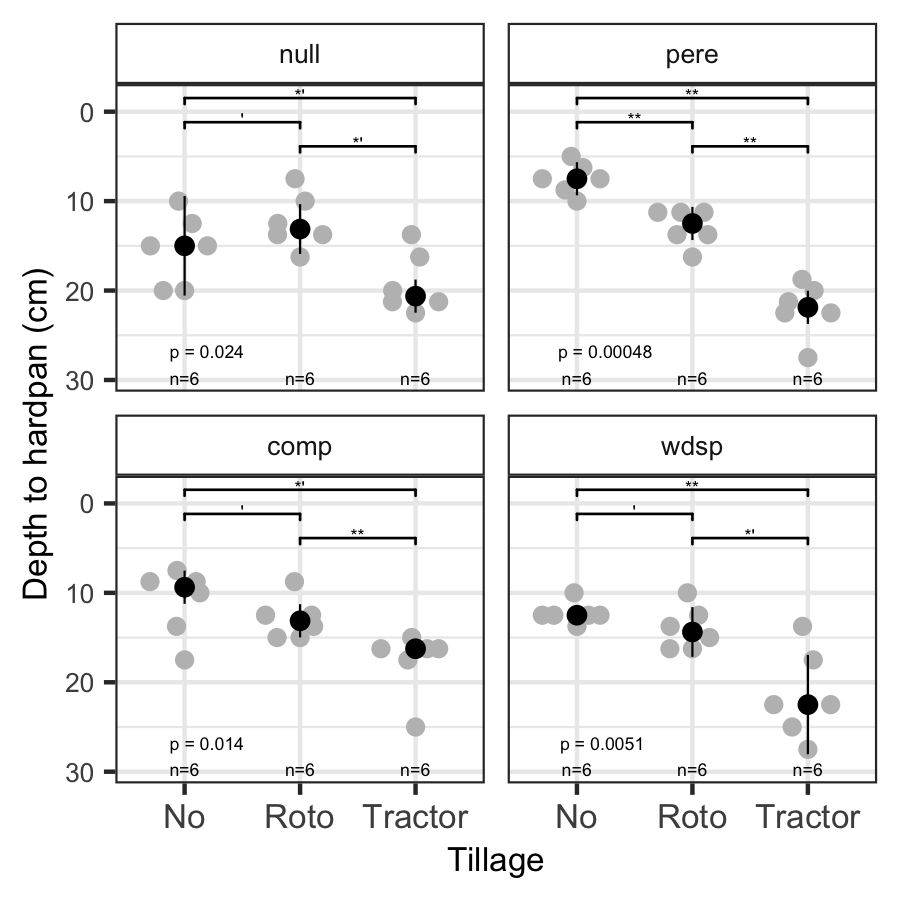
\includegraphics[width=12.5in]{../figs/compactionPlot} \caption{Compaction data}\label{fig:compactFig}
\end{figure}

There was also a significant interactive effect of tilling and cover crop mixtures (F6,59 = 3.88, p = 0.0025).
Broadly, tilling effects tended to be slightly more pronounced under the perennial mix compared to other crop mixes (\ref{fig:compactionFig}).
Furthermore, the perennial and compaction mixes both had notably lower compaction depths compared to the null mix, but these differences were only observed within the no-till group.
The perennial mix had the strongest effect, with an increase in compaction depth of 3 cm (\textasciitilde1'') (t59 = 4.62, p = 0.0001), and the compaction mix was associated with a change in compaction depth of 1.5 cm (\textasciitilde0.5'') (t59 = -2.6, p = 0.058).
Finally, there appeared to be more variation in compaction depth among crop mixes under no-till plots, which ranged 7-20 cm (3-8'') and included the most compacted plots, {[}whereas tilling tended to homogenize these cover crop effects{]}.
Finally, there were no general differences between sampling dates, though there was a tendency for compaction to increase slightly by 1-2.5 cm (0.5-1'') (F1,59 = 1.82, p = 0.183).

\hypertarget{infiltration-1}{%
\subsection{Infiltration}\label{infiltration-1}}

Soil infiltration was significantly affected by tillage across sampling times (p = 0.01) (Fig \ref{fig:infilFig}).
Roto-till showed significantly faster water infiltration rates compared to both no-till (pval) and tractor-till (pval), centering at \textasciitilde{}\textbf{\#\#\#} ± \textbf{\#\#\#} (conv\_), which was \textasciitilde{}\textbf{\#\#\#} (conv\_) faster than in both no-till and tractor-till plots.

In this case, season also very significantly affected infiltration (x22 = 15.02, p = 0.0001), with summer rates being 0.5-1 mL sec-1 (\textasciitilde0.5-1 gal hr-1) faster than autumn (dropping to \textasciitilde0.25 gal hr-1 or slower, beyond observation period), and early season rates appeared to underlie observed management effects (\ref{fig:infilFig}).

Cover crops only marginally significantly affected infiltration overall (\textbf{pvals}), and the weed suppression mix marginally significantly showed faster infiltration compared to null plots, speeding it up by \textbf{\#\#\#} up to \textbf{\#\#\#} ± \textbf{\#\#\#} mL per sec (\textbf{shown?}).

\begin{figure}
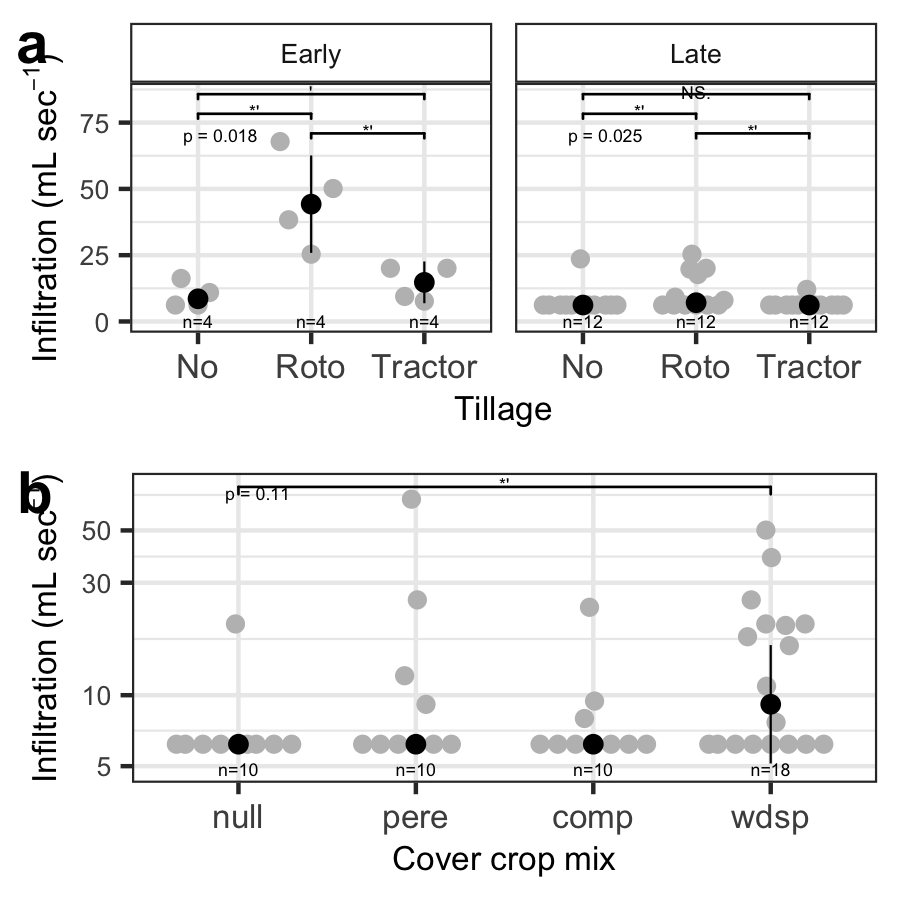
\includegraphics[width=12.5in]{../figs/infilPlot} \caption{Infiltration data}\label{fig:infilFig}
\end{figure}

\hypertarget{weed-density-and-richness}{%
\subsection{Weed density and richness}\label{weed-density-and-richness}}

Weed density was significantly affected by cover crop mix (x23 = 20.07, p = 0.0002) and significantly by the tillage method (x22 = 6.47, p = 0.04) (\ref{fig:weedsFig}).
Similarly, weed richness was significantly affected by cover crop mix (x23 = 30.97, p \textless{} 0.0001), yet not by tillage method (x22 = 1.64, p = 0.44) (\ref{fig:weedsFig}).
The weed suppression cover crop mix had the strongest effect on both weed species density and richness.
This mix of sorghum-sudangrass, buckwheat, and cowpea reduced the presence of the two focal common weeds, pigweed (\emph{Palmer amaranth}) and velvetleaf (\emph{Abutilon theophrasti}), regardless of tillage treatment.
The perennial cover crop mix seemed to show weed density that increased most consistently with tilling method intensity.

\begin{figure}
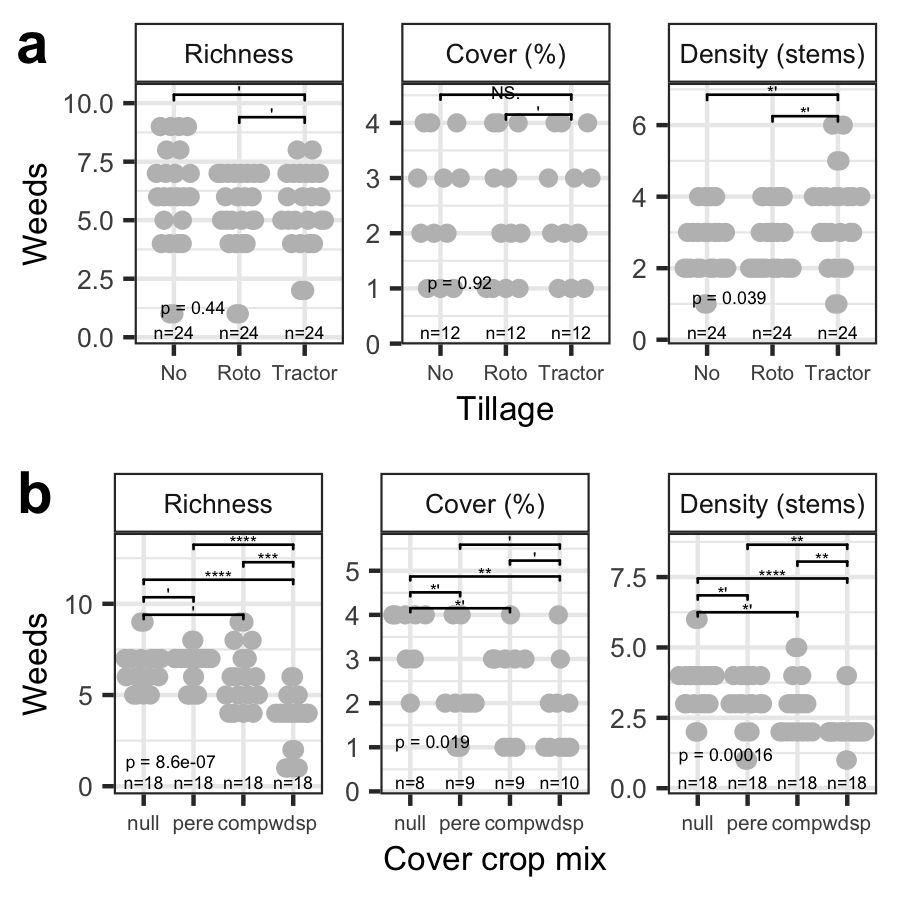
\includegraphics[width=12.5in]{../figs/weedPlot} \caption{Weeds data}\label{fig:weedsFig}
\end{figure}

We also monitored weed species presence and diversity in the spring of the following growing season, and the weed suppression mix plots had fewer early season weeds than the other plots as well (x23 = 10.00, p = 0.02; x22 = 0.17, p = 0.92).
From June to September, the other cover crop mixes did not significantly reduce weed pressure and actually performed similarly to our null group plots that only had weed seeds in them (\ref{fig:yieldFig}).
However, the wheat, rye, vetch, and clovers continued to grow from the Fall into the following Spring and did reduce weed presence compared to the null group in the spring.
Thus, although the other mixes did not reduce weeds in the summer or warm season, they were more effective at suppressing cool season weeds.

\hypertarget{radish-yield}{%
\subsection{Radish Yield}\label{radish-yield}}

Radish yield was not significantly affected by tillage (Fig \ref{fig:yieldFig}), and centered at \textasciitilde{}\textbf{\#\#\#} ± \textbf{\#\#\#} \emph{kg m\textsuperscript{-2}} and \textbf{\#\#\#} ± \textbf{\#\#\#} cm long.

However, radish plants did tend to grow the largest in no-till plots (Fig. 5). The longest radishes grew close to 21.6 cm or 8.5 inches, \ldots{} Forty percent of radishes sampled grew past the average compaction depth 11.43 cm (4.5 inches) in the no-till and tractor till plots.

\begin{figure}
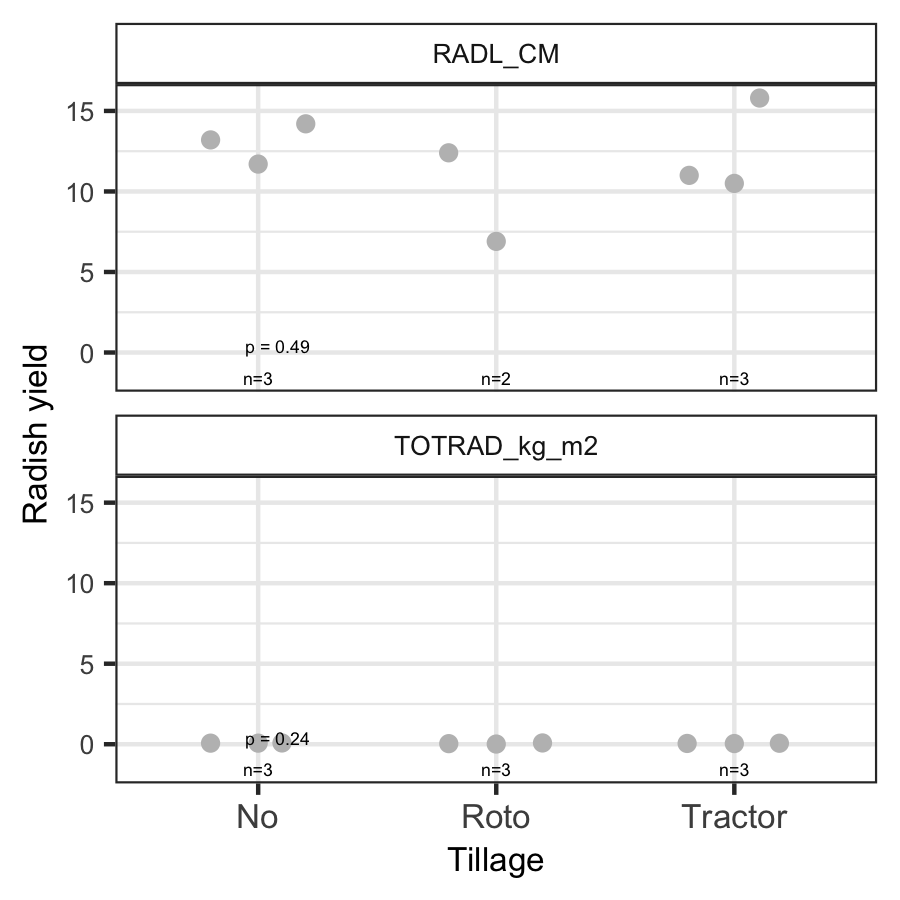
\includegraphics[width=12.5in]{../figs/yieldPlot} \caption{Yield data}\label{fig:yieldFig}
\end{figure}

\hypertarget{discussion}{%
\section{Discussion}\label{discussion}}

Overall this study informs urban soil management by supporting the use of tillage to address compaction issues and improve infiltration, together with cover crops to also reduce weed pressure.
We observed partial support for our hypothesis, in that tilling weakened compaction\ldots{}

Our data indicated that tilling significantly reduced compaction over a single growing season in both roto-tilled and tractor tilled plots \emph{(Fig. 1)}.
However, several no-till plots reached similar depths to rototilled plots, which suggests rototilling is not significantly more effective than no-till at reducing compaction.
Forage radish plant weight with foliage responded better in no-till plots that rototill and tractor tilled plots and average weights in the tilled groups were similar.
This was supported by detecting significantly higher radish yields in no-till compared to rototill and tractor till plots, while simultaneously measuring faster infiltration in rototill plots.
We also observed significant suppression of weed species diversity and overall density in the cover crop mix plots named for that targeted function, showing that the weed suppression mix used in this study can directly be applied in soils like these.

\hypertarget{tillage-1}{%
\subsection{Tillage}\label{tillage-1}}

Two reasons for tilling soil are reducing compaction and killing weeds.
In this experiment, both tractor and rototilling reduced compaction, loosening soil at lower depths than the no-till method \emph{(Fig. 2)}.
Tractor tilling with a subsoiler, moldboard plow, and rototiller likely created a high soil disturbance from the soil surface to depths as low as 30.48 cm or 12 inches.
The data show that greater levels of soil disturbance increased the density of the two most common weeds, velvet leaf (\emph{Abutilon theophrasti}) and pigweed (\emph{Palmer amaranth}), and decreased the diversity of other weed species \emph{(Fig. 4)}.

\hfill\break

The results show that the intensity of tillage corresponds negatively to compaction depth.
This effect also lasts throughout the growing season, even though the average depth of compaction tended to decrease over the growing season \emph{(Fig. 2)}.
Specifically, tractor tilled soils appeared to have a greater loss in compaction depth compared to no-till soils.
This is probably a combination of the natural tendency for clay soils to increase in compaction over time and weather conditions, limiting plant root penetration of soil to depths that would maintain soil looseness \emph{(Boswell et al.~2020)}.
Our data align with our previous predictions and other studies \emph{(Özpinar \& Çay, 2005)}.
Depending on what crops are grown, addressing compaction may not be an immediate issue.
Multiple crops have shallow root systems or are harvested before roots grow over 10.16 cm or 4 inches into the soil.
If crops do not require deep root systems, a no-till method may suffice \emph{(Krause \& Black, 1995)}, eliminating the time, energy, and costs of tilling.
An important observation for urban soil management was that rototilling and tractor tilling in particular exposed and removed debris from soil that would have remained in place with a no-till system.
The debris consisted of construction materials like rebar, wires, cables, bricks, cinder blocks, and pipes as well as other refuse.

\hfill\break

Finally, the reduction in compaction in the rototilled plots \emph{(Fig. 2)} may indicate that plant roots from both cover crops and weeds can reduce compaction.
Over multiple seasons, if crops with deep root systems are used, tilling may loosen soils at lower depths and facilitate deeper roots to establish more quickly than no-till.
Roots that penetrate to lower depths in soil allow plants to increase their access to nutrients and the water \emph{(Arshad, 1990)}.

\hypertarget{infiltration-2}{%
\subsection{Infiltration}\label{infiltration-2}}

Soil's ability to absorb water is critical for stormwater management, minimizing erosion, and making water available to plant roots.
Rototilled plots had the fastest infiltration early in the growing season \emph{(Fig. 3)}.
This coincides with predictions compared to no-till plots, but is the opposite of what we expected when compared to more deeply disturbed tractor tilled plots.
This may be explained by how compost was incorporated into the plots.

\hfill\break

For the no-till plots, compost was simply mulched on the surface, and after passing through this layer, water accumulated on the more compacted layer beneath.
In rototilled plots, compost was incorporated into the top six inches creating a more porous soil with organic matter throughout.
Compost in the tractor tilled plots was mixed in deeper than the other two treatments and may have become too sparse.
Thus, these more clayey soils were not porous enough to infiltrate water at high rates.
The infiltration rate decreased regardless of tillage treatment between the sampling dates, which was consistent with the pattern of increased compaction throughout the season.
The rate was so slow in the no-till and tractor till plots that these soils were draining less than one hundredth of a gallon in one minute.
This suggests that most water from a one inch rain event would result in runoff.
We posit that maintaining porosity and deeper compaction depths will allow soils to infiltrate water at rates that can absorb 2.54 cm or 1 inch rain events.
Based on our findings, rototilling and incorporating additional compost, may be an effective method to improve water infiltration during the driest time of year.
Rototilling disturbed the soil enough to reduce compaction, but not to the extent where organic matter was lost or highly dispersed.

\hypertarget{weed-suppression}{%
\subsection{Weed suppression}\label{weed-suppression}}

Overall weed density tended to be highest in tractor-tilled plots \emph{(Fig. 4)}.
This was likely due to increased soil disturbance exposing seeds in the soil seed bank and creating open space for weeds to emerge.
Higher weed density is an additional downside to the tillage of similar soils by tractor, along with lower infiltration rates.
Regardless of tillage treatment, the weed suppression mix of sorghum-sudangrass, buckwheat, and cowpea significantly reduced both weed density and species richness by more than a factor of two in some plots compared to the other cover crop mixes.
This result is supported by recommendations from other studies that pair buckwheat and sorghum-sudangrass \emph{(Smith et. al, 2015)}.
Weed richness may have decreased due to competitive exclusion by sorghum-sudangrass via allelopathy, and by buckwheat via better phosphorus mining and use \emph{(Jabran 2017; Zhu et al.~2002)}.

\hfill\break

The weed suppression mix can be utilized to frame crop beds, keeping out encroaching weeds, or to reduce weed pressure in an area that will be planted in the fall or following season.
The buckwheat and sorghum-sudan grass grows quickly in poor soils and even dry conditions.
These plants accumulate a lot of biomass, which allows them to shade out weeds.
They also can be mowed to prevent re-seeding and winter-kill, making them easier crops to manage than crops that require more maintenance.
This experiment was designed to require no management after seeding (i.e.~no irrigation, weeding, or mowing).
Under these conditions, most of the cover crops did not perform well, and were probably inhibited by the warm and dry summer conditions.
Crops in other mix treatments used here usually prefer to be sown in the cooler early season \emph{(United States Department of Agriculture, 2015)}.
This experiment highlighted crops could be used in clayey soils under these conditions: forage radish, buckwheat, cowpea, and sorghum-sudangrass.
Aside from reducing weeds for crop production, weed suppression can reduce pollen counts and the likelihood of direct contact with people \emph{(Katz et al.~2014; Katz \& Carey 2014)}.
In urban areas this has implications for serving communities where asthma and respiratory illness is common, as well as preventing exposure to weeds that may cause irritation.
Under managed landscapes could have cover crops sowed to alleviate some of these urban issues.

\hypertarget{yield-and-root-length}{%
\subsection{Yield and root length}\label{yield-and-root-length}}

Forage Radish tended to grow the most in no-till plots, which was unexpected based on the higher compaction in these plots.
We posit that the radishes benefited from having more access to the nutrients in the compost that was simply mulched on the top two inches of the no-till plots.
The compost in the other tillage treatments was incorporated throughout the soil of other plots and less available.
It was also surprising that yield did not correspond with faster infiltration, since no-till plots had slower infiltration compared to rototilled plots.
This suggests a more nuanced relationship between infiltration and root crop yield unlike the relationship between infiltration and compaction.
Yield responds more to more stable or longer-term reservoirs of water and nutrients, such as those in mulched compost, than to shorter-term or more transient influxes brought by infiltration processes \emph{(Schlegel \& Havlin 2017)}.
Furthermore, more stable reservoirs of water and nutrients may also foster more productive associations with soil microbes, which serve as an additional source of available nutrients for plant roots.
In these cases, soil microbe availability might depend less on pH.
These data suggest that similar alternative soil management practices like no-till combined with compost and mulching application gives better yields.
Thus, forage radish can be an effective cover crop in reducing compaction and building soil structure, with minimal or no mechanical tillage \emph{(Chen, 2010)}.
Our study also warrants future studies on the processes tying yield to land management in similar soils.

\newpage

\hypertarget{references}{%
\section*{References}\label{references}}
\addcontentsline{toc}{section}{References}

\hypertarget{refs}{}
\begin{CSLReferences}{1}{0}
\leavevmode\vadjust pre{\hypertarget{ref-beniston16}{}}%
Beniston, Joshua W., Rattan Lal, and Kristin L. Mercer. 2016. {``Assessing and {Managing Soil Quality} for {Urban Agriculture} in a {Degraded Vacant Lot Soil}.''} \emph{Land Degradation and Development} 27 (4): 996--1006. \url{https://doi.org/10.1002/ldr.2342}.

\leavevmode\vadjust pre{\hypertarget{ref-king20}{}}%
King, Alison E., Genevieve A. Ali, Adam W. Gillespie, and Claudia Wagner-Riddle. 2020. {``Soil {Organic Matter} as {Catalyst} of {Crop Resource Capture}.''} \emph{Frontiers in Environmental Science} 8 (May). \url{https://doi.org/10.3389/fenvs.2020.00050}.

\leavevmode\vadjust pre{\hypertarget{ref-kumar16}{}}%
Kumar, Kuldip, and Lakhwinder S. Hundal. 2016. {``Soil in the {City}: {Sustainably Improving Urban Soils}.''} \emph{Journal of Environmental Quality} 45 (1): 2--8. \url{https://doi.org/10.2134/jeq2015.11.0589}.

\leavevmode\vadjust pre{\hypertarget{ref-kuzyakov19}{}}%
Kuzyakov, Yakov, and Kazem Zamanian. 2019. {``Reviews and Syntheses: {Agropedogenesis} \textendash{} Humankind as the Sixth Soil-Forming Factor and Attractors of Agricultural Soil Degradation.''} \emph{Biogeosciences} 16 (24): 4783--803. \url{https://doi.org/10.5194/bg-16-4783-2019}.

\leavevmode\vadjust pre{\hypertarget{ref-montgomery07}{}}%
Montgomery, David R. 2007. {``Soil Erosion and Agricultural Sustainability''} 104 (33): 13268--72.

\leavevmode\vadjust pre{\hypertarget{ref-oldfield19}{}}%
Oldfield, Emily E., Mark A. Bradford, and Stephen A. Wood. 2019. {``Global Meta-Analysis of the Relationship Between Soil Organic Matter and Crop Yields,''} 15--32.

\leavevmode\vadjust pre{\hypertarget{ref-small19}{}}%
Small, Gaston, Paliza Shrestha, Geneviève Suzanne Metson, Katherine Polsky, Ivan Jimenez, and Adam Kay. 2019. {``Excess Phosphorus from Compost Applications in Urban Gardens Creates Potential Pollution Hotspots {Excess} Phosphorus from Compost Applications in Urban Gardens Creates Potential Pollution Hotspots.''}

\leavevmode\vadjust pre{\hypertarget{ref-stewart07}{}}%
Stewart, Catherine E., Keith Paustian, Richard T. Conant, Alain F. Plante, and Johan Six. 2007. {``Soil Carbon Saturation: Concept, Evidence and Evaluation.''} \emph{Biogeochemistry} 86 (1): 19--31. \url{https://doi.org/10.1007/s10533-007-9140-0}.

\end{CSLReferences}

\end{document}
